\section{Results}
\label{sec:results}

\subsection{All models drop on lab-confirmed photographs}
\label{sec:res-bench}

Table~\ref{tab:bench} and Figure~\ref{fig:bench} compare every model on the two test sets. On the farm test all of
them are in the range earlier work reports. MobileNetV2 calls 99.6\% of the 679 photographs correctly \todo{mean over
seeds}, and our detector 98.5\% when it always gives its best guess. On the 1,255 lab-confirmed photographs every model
loses more than 20 points. MobileNetV2 falls to 74.6\% and the detector to 76.3\% \todo{final means and ranges}. The
Wilson intervals of the two test sets do not overlap for any model, so the drop is not sampling noise.

Our detector does not classify better than the classifiers earlier work used. The differences between models on the
lab-confirmed photographs are small next to the drop that every model shows. Under this protocol the published
accuracies of 98 to 99\% describe photographs like the training photographs, and the choice of architecture matters
less than the choice of test set.

\begin{table}[t]
\centering
\caption{Accuracy and macro-F1 on the held-out farm test (679 photographs) and the lab-confirmed photographs (1,255),
for models trained on the same 5,451 photographs. Classifiers: mean over three seeds, range in brackets.
Detector: one run, scored with its best class in each photograph (always answers) and with the deployed 0.25
confidence threshold (below it the photograph counts as wrong).}
\label{tab:bench}
\small
\begin{tabular}{lcccc}
\toprule
& \multicolumn{2}{c}{Farm test} & \multicolumn{2}{c}{Lab-confirmed} \\
Model & Accuracy & Macro-F1 & Accuracy & Macro-F1 \\
\midrule
MobileNetV2~\cite{machuve2022} & \todo{} & \todo{} & \todo{} & \todo{} \\
EfficientNet-B0~\cite{dhungana2025} & \todo{} & \todo{} & \todo{} & \todo{} \\
ResNet-50 & \todo{} & \todo{} & \todo{} & \todo{} \\
YOLO11n (ours), always answers & 98.5 & 98.3 & 76.3 & 75.1 \\
YOLO11n (ours), 0.25 threshold & 97.9 & 97.7 & 67.1 & 70.3 \\
\bottomrule
\end{tabular}
\end{table}

\begin{figure}[t]
\centering
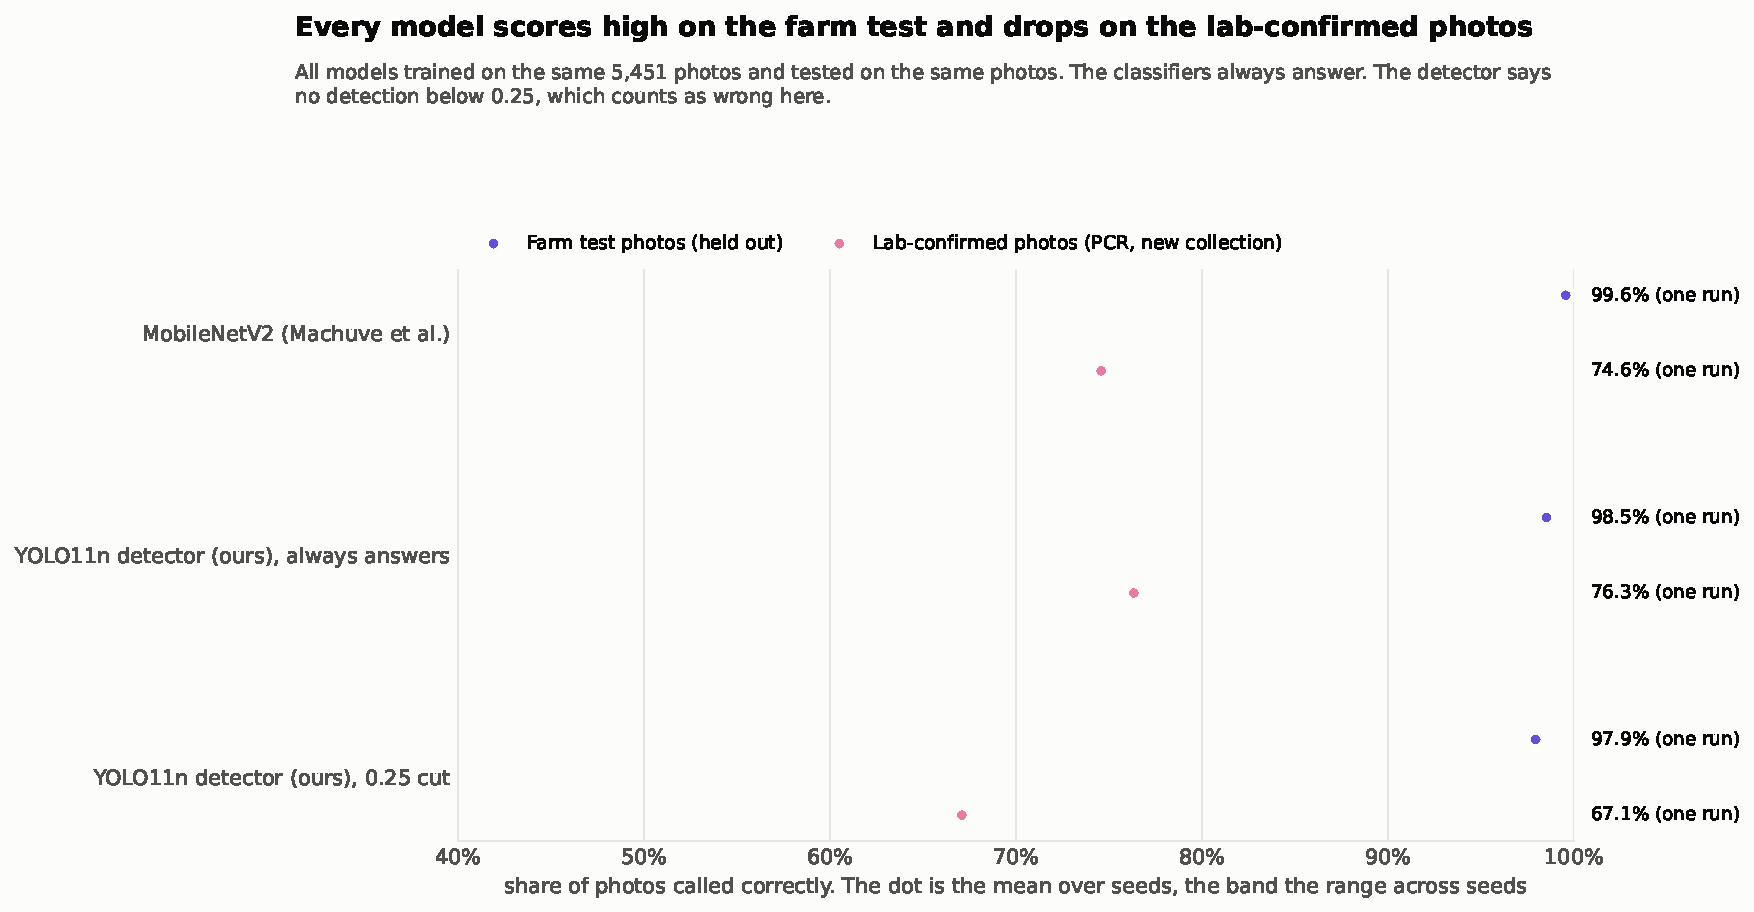
\includegraphics[width=\linewidth]{figures/13_benchmark.pdf}
\caption{Accuracy of each model on the farm test and on the lab-confirmed photographs. Dots are the mean over seeds,
bands the range across seeds. Values are written beside each mark.}
\label{fig:bench}
\end{figure}

\subsection{Where the errors go}
\label{sec:res-errors}

Figure~\ref{fig:confusion} shows the detector's calls on both sets. On the farm test the diagonal holds 95 to 100\% of
every class. On the lab-confirmed photographs most errors are not confusions between diseases. They are photographs
with no detection at all (20\% of healthy and 27\% of Newcastle-like photographs) and photographs called healthy or
salmonella-like by mistake. Newcastle-like recall falls the most, from 94.6\% (35 of 37) to 41.9\% (78 of 186). This
class has 376 photographs in the whole farm collection, against more than 2,000 for each of the others
(Figure~\ref{fig:recall}).

\begin{figure}[t]
\centering
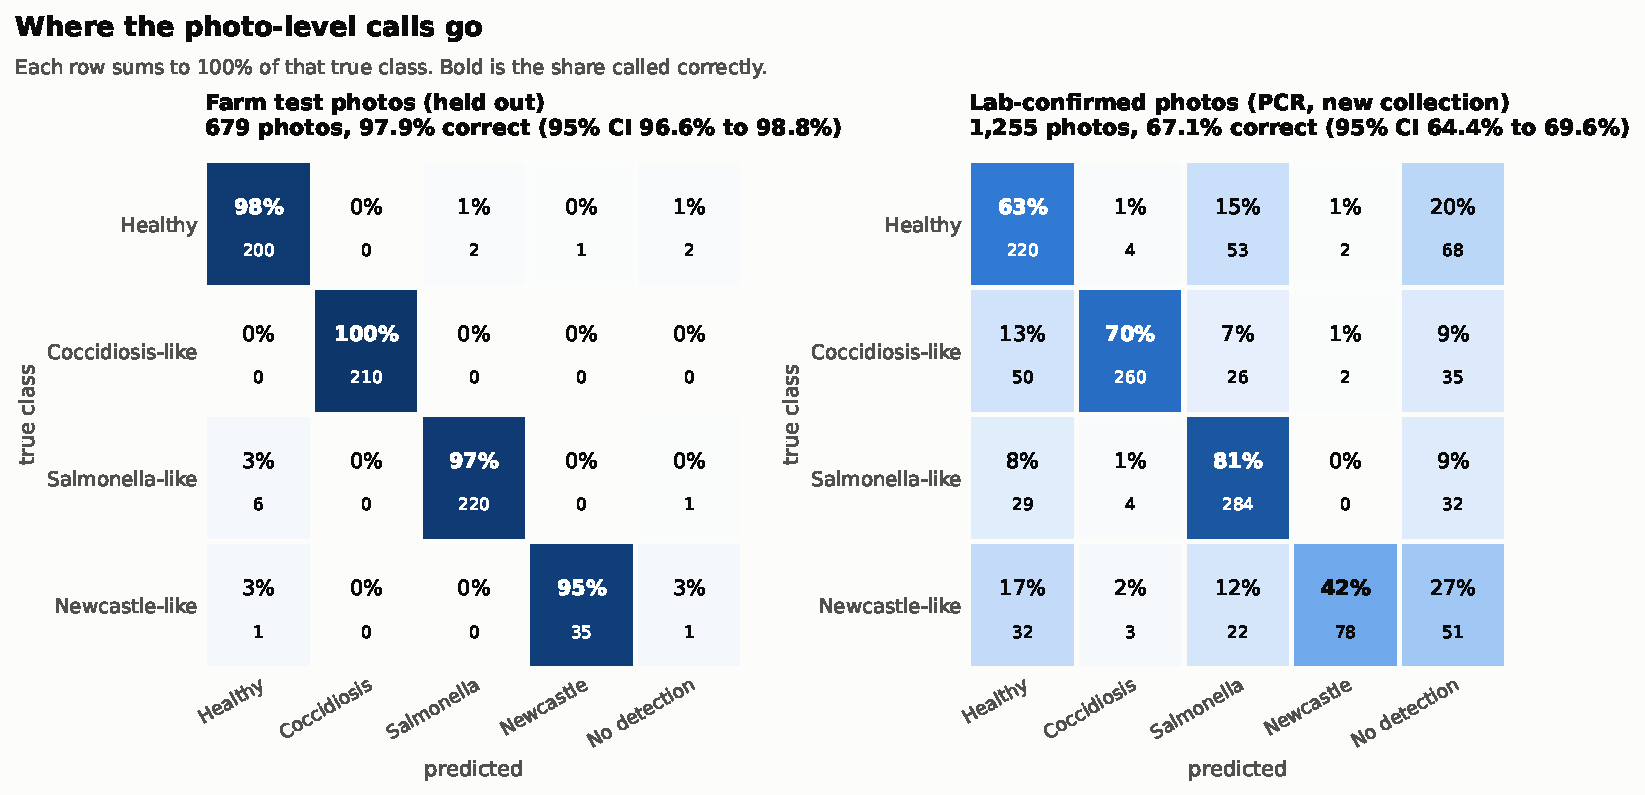
\includegraphics[width=\linewidth]{figures/06_confusion_matrices.pdf}
\caption{Detector calls per true class on the farm test (left) and the lab-confirmed photographs (right). Each row
sums to 100\%. Counts under each share.}
\label{fig:confusion}
\end{figure}

\begin{figure}[t]
\centering
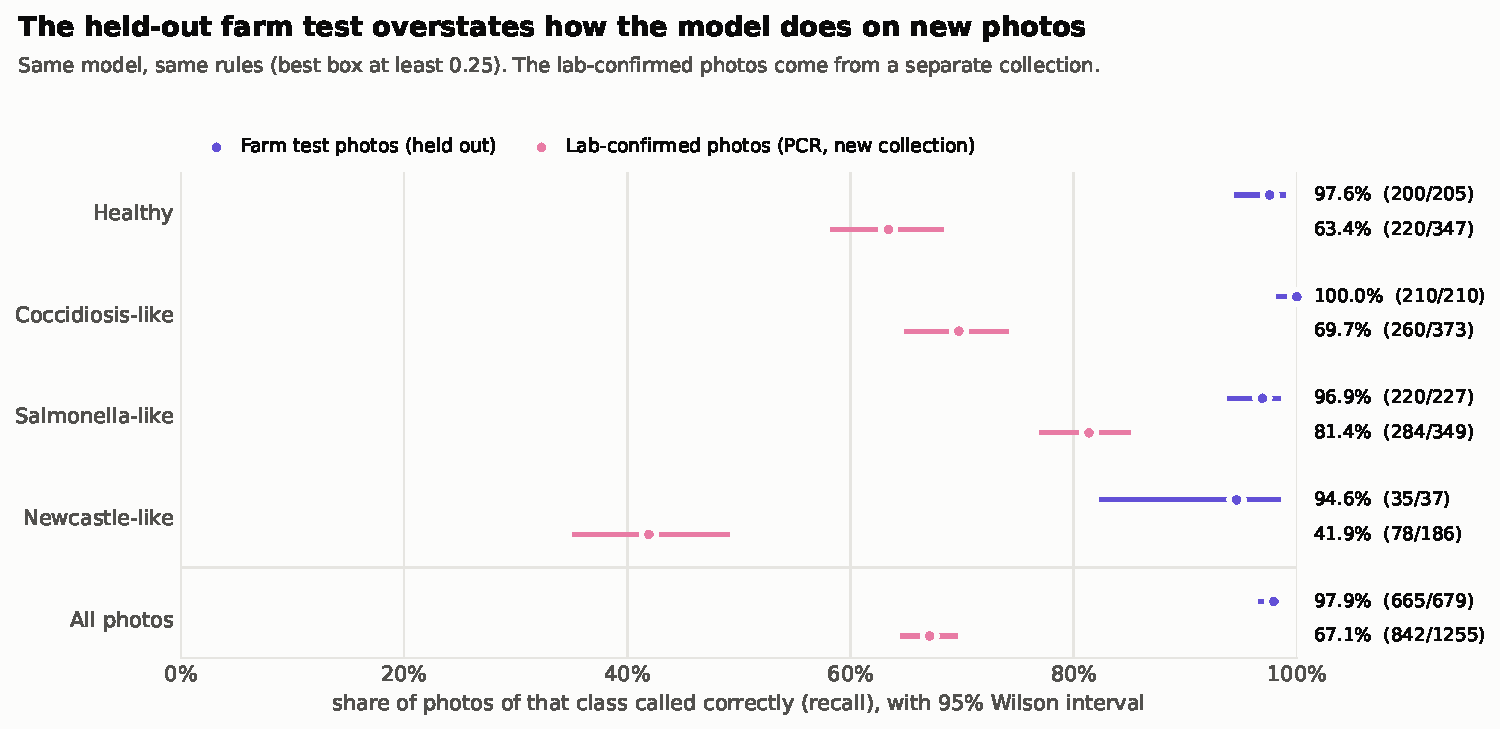
\includegraphics[width=\linewidth]{figures/07_recall_by_class.pdf}
\caption{Per-class recall of the detector with 95\% Wilson intervals, at the deployed 0.25 threshold.}
\label{fig:recall}
\end{figure}

\subsection{Duplicates do not explain the farm score}
\label{sec:res-dup}

Forty-nine of the 679 farm test photographs (7.2\%) have a training photograph with an identical 256-bit difference
hash, and inspection of the closest pairs shows they are the same image saved under two file names
(Figure~\ref{fig:dup}). Every other test photograph differs from its nearest training photograph in at least 40
bits. The detector calls all 49 copies correctly. Without them its farm accuracy is 97.8\% (95\% CI 96.3 to 98.7\%),
against 97.9\% with them. The copies are a flaw in the split, but they are not why the farm test overstates
performance on new photographs.

\begin{figure}[t]
\centering
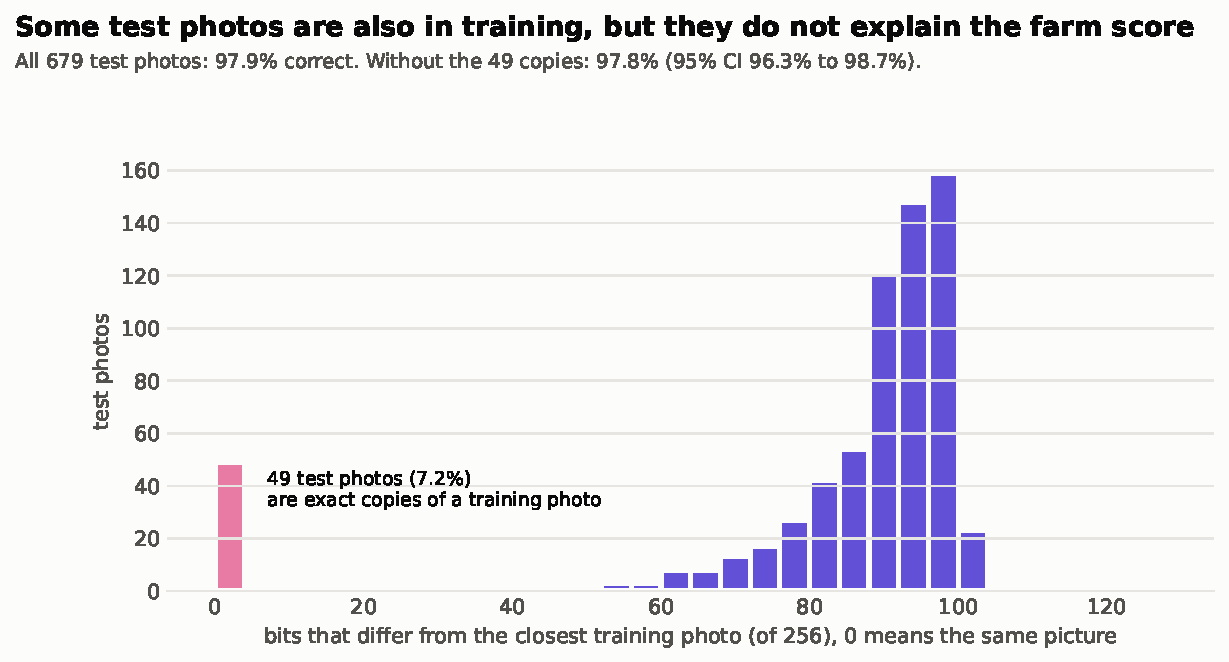
\includegraphics[width=\linewidth]{figures/10_duplicates_across_split.pdf}
\caption{Hamming distance from each farm test photograph to its nearest training photograph (256-bit difference
hash). The bar at zero holds the 49 exact copies.}
\label{fig:dup}
\end{figure}

\subsection{The box score ranks well but is not a probability}
\label{sec:res-cal}

If the detector only answers when its best box clears a threshold, its answers become more reliable
(Figure~\ref{fig:coverage}). On the lab-confirmed photographs, raising the threshold from 0.25 to 0.80 raises the
accuracy of the answers from 78.8\% to 87.4\%, but the detector then answers only 27.8\% of photographs. Its scores
are also under-confident on both sets (Figure~\ref{fig:calibration}). The expected calibration error is 0.177 on the
farm test and 0.172 on the lab-confirmed photographs, and in both cases the photograph is right more often than the
score says. The score should therefore be calibrated, for example by temperature scaling~\cite{guo2017} on the
validation split, before it is shown to a farmer as a percentage.

\begin{figure}[t]
\centering
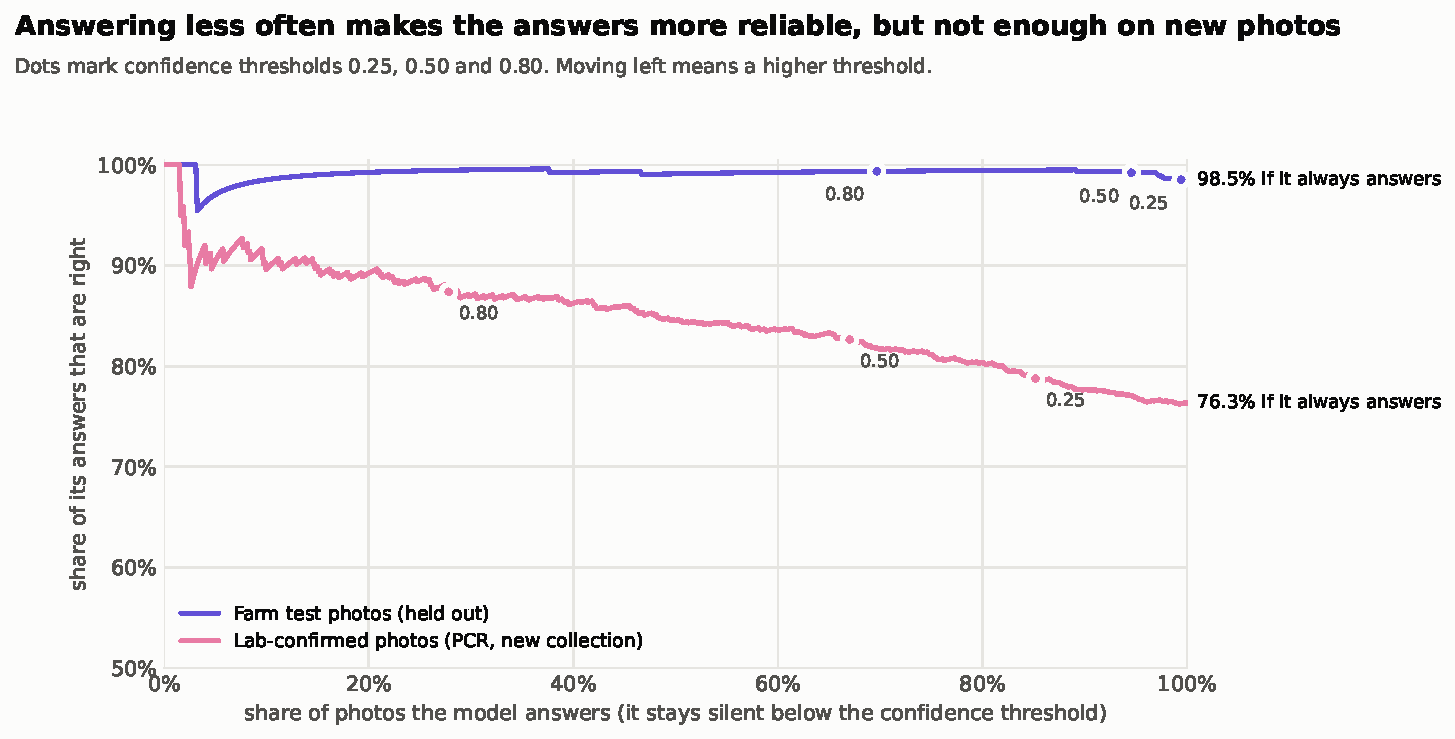
\includegraphics[width=\linewidth]{figures/08_accuracy_vs_coverage.pdf}
\caption{Accuracy of the detector's answers against the share of photographs it answers, as the confidence threshold
rises. Dots mark the thresholds 0.25, 0.50 and 0.80.}
\label{fig:coverage}
\end{figure}

\begin{figure}[t]
\centering
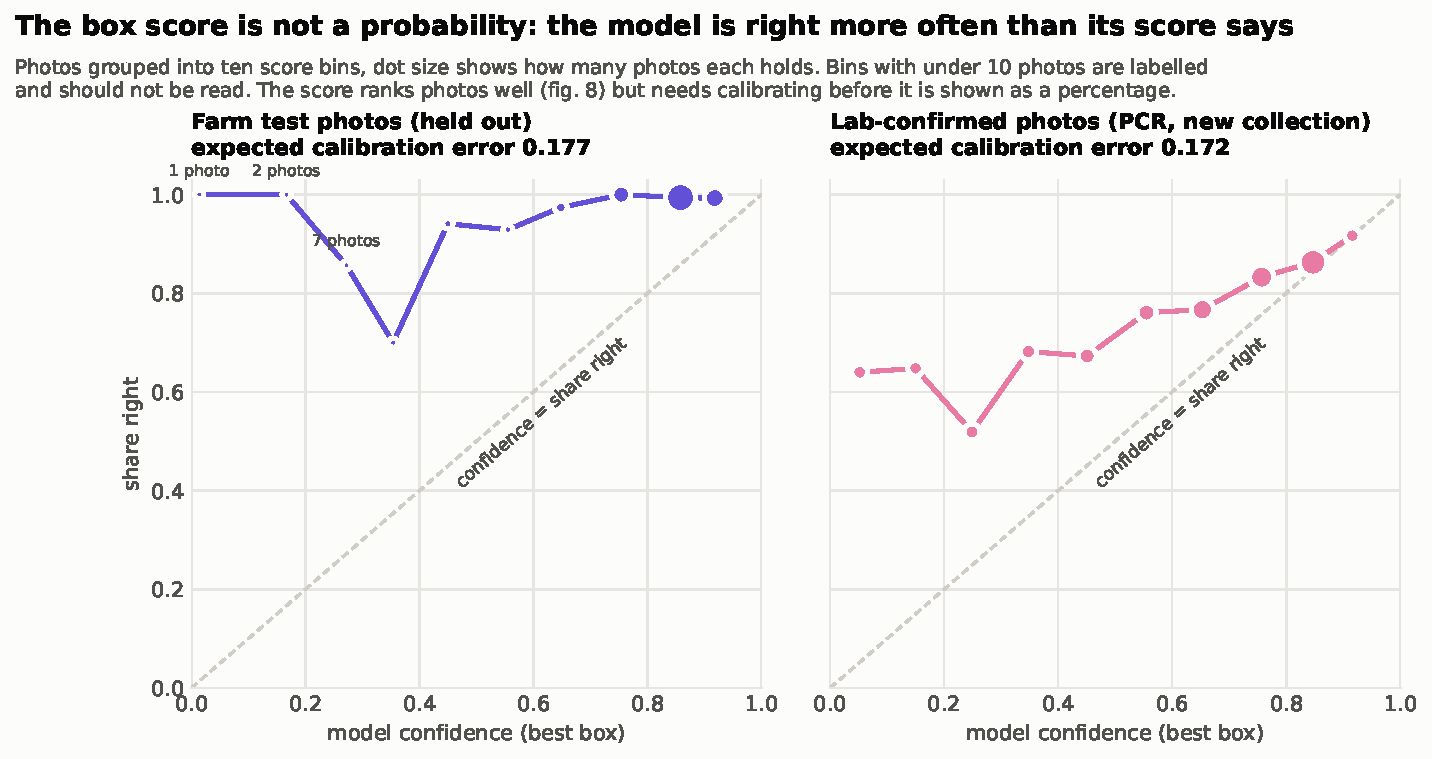
\includegraphics[width=\linewidth]{figures/09_calibration.pdf}
\caption{Reliability diagrams over ten score bins. Dot size shows the number of photographs in a bin. Bins with fewer
than ten photographs are labelled and should not be read.}
\label{fig:calibration}
\end{figure}

\subsection{Pen-scale detection}
\label{sec:res-pen}

The close-up detector does not work at pen scale (Figure~\ref{fig:pen}). On the held-out pen cameras it finds 29\% of
droppings, only 11\% of its boxes are droppings, and it places 3.55 boxes on an average empty pen tile at the 0.25
threshold. After pen-scale fine-tuning, recall is 0.80 and precision 0.93 on cameras the model never saw, and false
boxes on empty tiles fall to 0.05 per tile. The close-up mAP50 changes from 0.873 to 0.853. Class accuracy at pen
size remains weaker than detection (four-class mAP50 0.65). The pen model should therefore find a dropping, and a
full-resolution patch or a close-up photograph should be judged by the close-up model.

\begin{figure}[t]
\centering
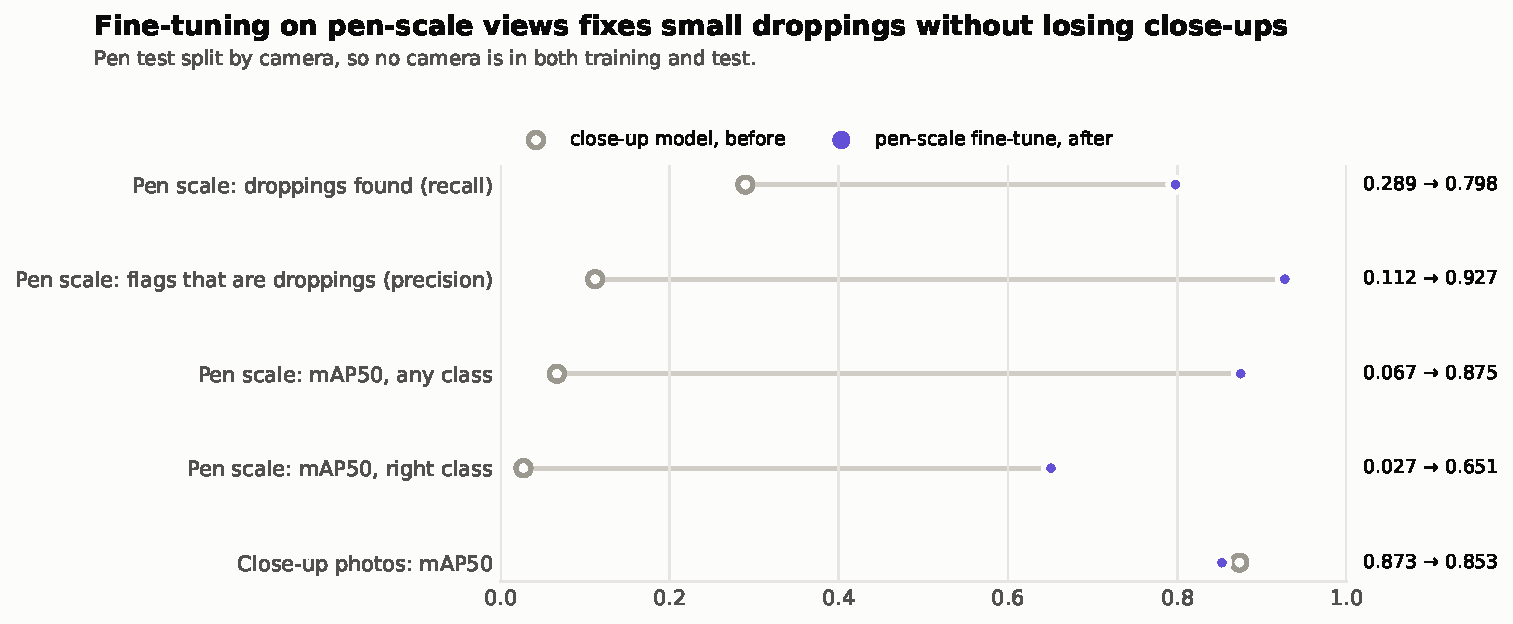
\includegraphics[width=\linewidth]{figures/11_pen_scale_before_after.pdf}
\caption{Pen-scale test on held-out cameras before (close-up model) and after fine-tuning. The pen test uses real
droppings pasted onto real litter.}
\label{fig:pen}
\end{figure}

Whole-photograph classifiers cannot be tested this way. They return one label for an image, and in a pen frame a
dropping covers at most about 0.1\% of the image. Locating the dropping is what makes the pen camera usable, and it is
the main reason to use a detector in this setting rather than a better classifier.

\subsection{The deployed pipeline}
\label{sec:res-qnx}

We also ran the pen model over a three-minute clip from the held-out PIO camera, into which ten test droppings were
pasted at known times. Read at two frames a second with a short persistence rule, it flagged seven, five of them
within two seconds of their appearance, and raised no false flags (Figure~\ref{fig:live}). This run was made on a
laptop, and like the pen test it uses pasted droppings. On the Pi, the deployed pipeline proposes candidates with a
still-spot finder and judges a full-resolution patch of each with the close-up detector. On the Raspberry Pi
5 the detector takes 168\,ms at 320 pixels and 618\,ms at 640 pixels with four threads, and the pen model 608\,ms at
640 pixels \todo{full timing table for all models under the same harness}. Native message passing between two
sections takes 95\,$\mu$s for a 57.6\,KB frame and reply. When we killed any section with \texttt{SIGKILL}, the
supervisor restarted it in 20 to 33\,ms. Killing the spot finder cost the camera one frame and the other sections
none.

\begin{figure}[t]
\centering
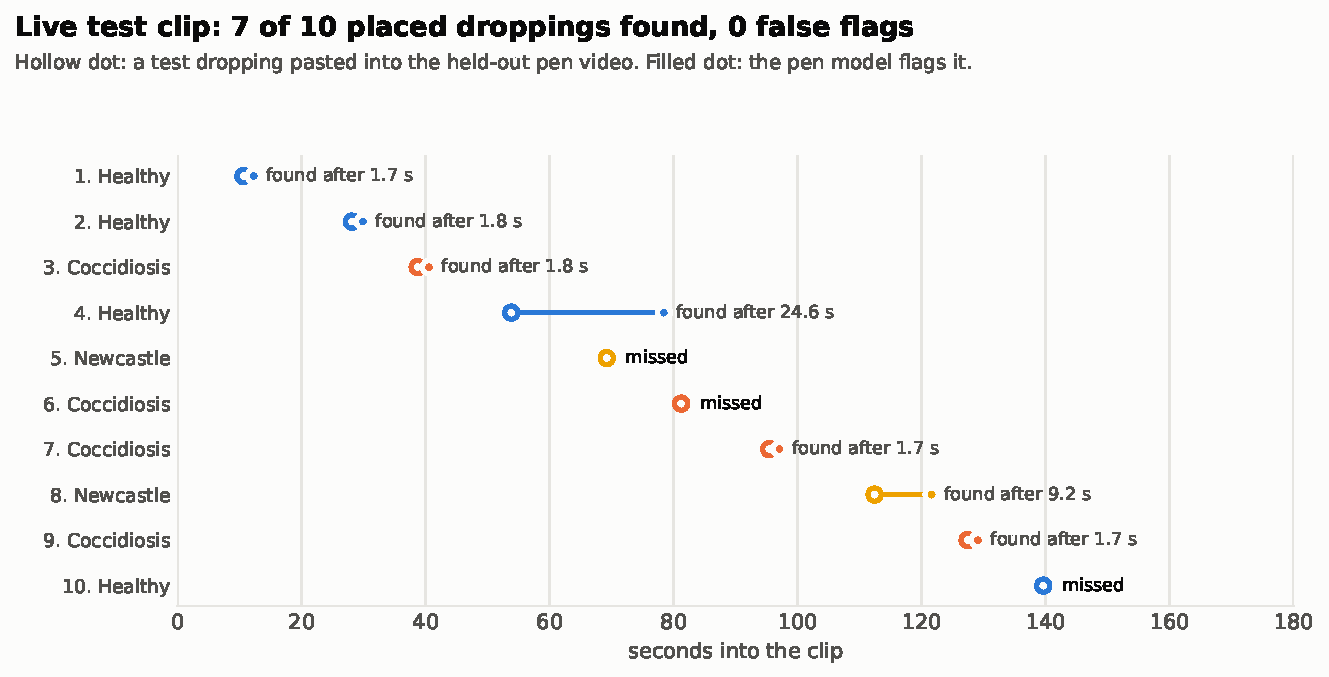
\includegraphics[width=\linewidth]{figures/12_live_clip_answer_key.pdf}
\caption{Test clip with an answer key. Hollow dots mark when each pasted dropping appears in the held-out video,
filled dots when the pen model flagged it.}
\label{fig:live}
\end{figure}
